\begin{figure}[htbp]
    \centering
    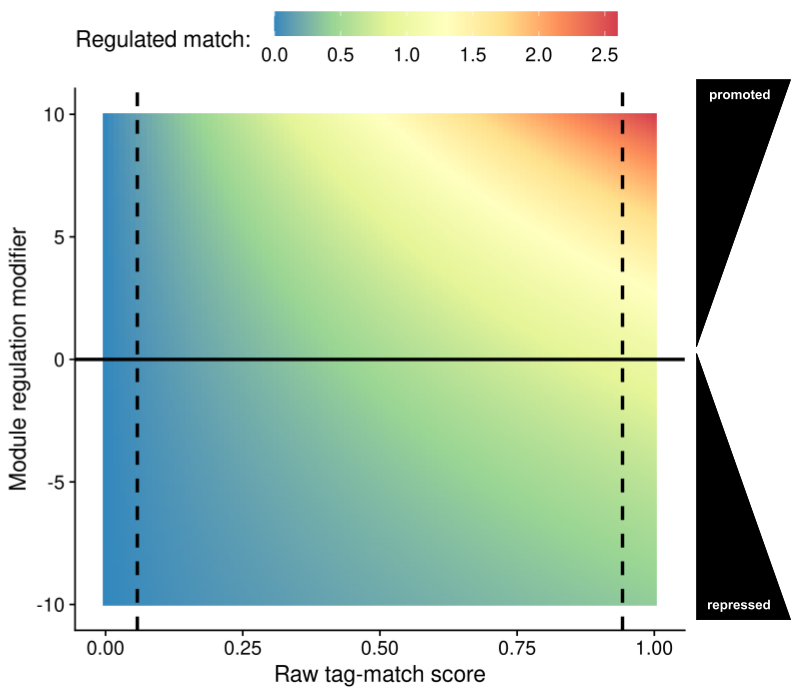
\includegraphics[width=0.6\columnwidth]{chapters/05-tag-based-genetic-regulation/media/expontential-regulation.png}
    \caption{\small
    \textbf{Regulated tag-match score as a function of raw tag-match score and regulatory modifier values according to Equation \ref{chapter:tag-based-regulation:equ:reg-transform}.}
    The horizontal black line indicates a neutral regulatory state; 
    repressed states are below the line, and promoted states are above the line.
    We expect the raw tag-match score (calculated using the Streak similarity metric, which is described later in Section \ref{chapter:tag-based-regulation:sec:methods:signalgp}) of 90\% of random pairs of tags to fall between the two dashed vertical lines; to compute the location of these lines, we generated $10^{5}$ pairs of random tags and found the region that contained the middle 90\% of raw tag-matching scores.
    }
    \label{chapter:tag-based-regulation:fig:exponential-regulation-function}
\end{figure}